% !TeX program = pdflatex
% -------------------------------------------------------------------------
%  crowbar_bidir.tex
%  Bidirectional self-triggered thyristor crowbar for bypass protection of a
%  low-impedance element: concept, coordination, functional Simscape model.
%  Conventions: English, thebibliography (no biblatex), no babel, no lmodern.
% -------------------------------------------------------------------------
\documentclass[11pt,a4paper]{article}

\usepackage[T1]{fontenc}
\usepackage[utf8]{inputenc}
\usepackage[margin=25mm]{geometry}
\usepackage{amsmath,amssymb}
\usepackage{siunitx}
\usepackage{booktabs}
\usepackage{graphicx}
\usepackage{caption}
\usepackage[european]{circuitikz}
\usetikzlibrary{arrows.meta}
\usepackage{fancyhdr}
\usepackage[hidelinks]{hyperref}

% ---------------- document identification / revision ----------------------
\newcommand{\doctitle}{Bidirectional Self-Triggered Thyristor Crowbar}
\newcommand{\docsubtitle}{Bypass Protection of a Low-Impedance Element in the 3~kV / 3600~A Bench: Concept, Coordination and Functional Simscape Model}
\newcommand{\docrev}{00}
\newcommand{\docdate}{2026-09-12}
\newcommand{\docid}{crowbar\_bidir}

\pagestyle{fancy}
\fancyhf{}
\lhead{\small \docid}
\rhead{\small Rev.~\docrev}
\lfoot{\small \docdate}
\cfoot{\small \thepage}
\renewcommand{\headrulewidth}{0.4pt}

\sisetup{per-mode=symbol, range-phrase=--, range-units=single}

\title{\textbf{\doctitle}\\[6pt]\large \docsubtitle\\[10pt]\normalsize Rev.~\docrev\ --- \docdate}
\author{}
\date{}

\begin{document}
\maketitle
\thispagestyle{fancy}

\begin{center}
\begin{tabular}{@{}llp{9.5cm}@{}}
\toprule
\textbf{Rev.} & \textbf{Date} & \textbf{Description} \\
\midrule
00 & 2026-09-12 & First issue. Concept, coordination rules, worked example, Simscape component \texttt{crowbar\_bidir}. \\
\bottomrule
\end{tabular}
\end{center}

\begin{abstract}
An element that is structurally a short circuit (a few volts at the full \SI{3600}{A}) sits in
the current path of the \SI{3}{kV} inductive test bench. If it opens, the loop inductance drives
its terminal voltage up without limit. This note describes a bidirectional, fully passive
thyristor crowbar placed in parallel with the element: two antiparallel thyristors, each fired
by a floating break-over network, that short the element within a few microseconds in either
polarity. The differences with respect to the unidirectional dump crowbar of the load are
worked out: one thyristor is always forward biased in service, the voltage rise at opening is
essentially unlimited, and the crowbar becomes a permanent short that must be cleared by the
main switch. Coordination rules for the snubber capacitor, the MOV, the series reactor, the
firing level and the thermal duty are given with a worked example, followed by the description
of a functional Simscape component, \texttt{crowbar\_bidir}, and a test procedure.
\end{abstract}

% ==========================================================================
\section{Purpose and scenario}
% ==========================================================================

The bench of Fig.~\ref{fig:system} circulates $I_0 = \SI{3600}{A}$ in an RL load
($R = \SI{0.8}{\ohm}$, $L = \SI{2}{mH}$) from a \SI{3}{kV} source through a static switch $S$;
the load energy at opening is extracted by the dump crowbar described in
\texttt{crowbar\_thyristor\_selftrigger}. A further element $E$ is inserted in series in the
loop. In service $E$ is a low-impedance path: with $R_E \approx \SI{1.4}{m\ohm}$ it drops
about \SI{5}{V} at full current. Should $E$ open, whether by failure or by an unwanted
command, the loop current has no path and the voltage across $E$ rises at
\begin{equation}
  \frac{\mathrm{d}v_E}{\mathrm{d}t} = \frac{I_0}{C_{par}},
  \label{eq:dvdt_par}
\end{equation}
where $C_{par}$ is whatever capacitance hangs on its terminals: with a few nanofarads this is
hundreds of \si{V/ns}. The requirement is a device in parallel with $E$ that turns into a
short circuit as soon as $v_E$ exceeds a threshold, in either polarity, without auxiliary
supply, and stays shorted until the main switch clears the current.

\begin{figure}[htbp]
\centering
\begin{circuitikz}[american, scale=0.9, transform shape]
  % source
  \draw (0,0) to[battery1, l_=$V_s$] (0,4);
  \node[font=\scriptsize] at (0.35,3.35) {$+$};
  \node[font=\scriptsize] at (0.35,0.65) {$-$};
  % switch with MOV
  \draw (0,4) -- (1,4) to[nos, l=$S$] (3,4) -- (4,4);
  \draw (1,4) -- (1,5.3) to[varistor, l=MOV] (3,5.3) -- (3,4);
  % element E with bypass crowbar
  \draw (4,4) to[generic, l=$E$] (7,4) -- (8.5,4);
  \draw (4,4) -- (4,2.3) -- (4.6,2.3);
  \draw (7,4) -- (7,2.3) -- (6.4,2.3);
  \draw[thick] (4.6,1.5) rectangle (6.4,3.1);
  \node[align=center, font=\scriptsize] at (5.5,2.3) {bidirectional\\crowbar\\(Fig.~\ref{fig:crowbar})};
  \draw[-latex] (4.3,3.6) -- (4.9,3.6) node[midway, above, font=\scriptsize] {$i_E$};
  % load
  \draw (8.5,4) to[R, l_=$R$] (8.5,2.5) to[L, l_=$L$] (8.5,0.5) -- (8.5,0) -- (0,0);
  % dump crowbar (simplified)
  \draw (8.5,4) -- (10.5,4) to[R, l_=$R_D$] (10.5,2.6) to[L, l_=$L_c$] (10.5,1.7) to[Ty, l_=$T_D$, invert] (10.5,0) -- (8.5,0);
  \node[font=\scriptsize, align=center, anchor=west] at (10.9,3.3) {load dump\\crowbar};
\end{circuitikz}
\caption{Bench with the low-impedance element $E$ in the source branch and its bidirectional
bypass crowbar. $E$ may equally sit inside the load loop; the position changes the transient
voltage seen in service (Section~\ref{sec:vst}).}
\label{fig:system}
\end{figure}

Three features distinguish this crowbar from the dump crowbar of the load:

\begin{enumerate}
\item \textbf{Bias in service.} The dump thyristor is reverse biased at \SI{-3}{kV} all the
      time and sees forward voltage only when it must fire. Here $v_E \approx \SI{5}{V}$, so one
      of the two antiparallel thyristors is \emph{always} forward biased, at low voltage, and
      exposed to whatever transient $E$ develops. Immunity to false firing is a design
      requirement, not a by-product.
\item \textbf{Voltage rise.} At the dump crowbar the forward voltage is bounded by the MOV of
      the switch. Here nothing bounds $v_E$ except what is deliberately placed across $E$: the
      time between the opening and the thyristor conduction (\SIrange{1}{3}{\micro s}) must be
      covered by a capacitor and a MOV.
\item \textbf{Duty after firing.} The dump crowbar carries a decaying current and turns off by
      itself. The bypass crowbar shorts $E$ while the source keeps driving the loop: it carries
      $I_0$ continuously until $S$ opens. It is a latch, and its firing must trip $S$.
\end{enumerate}

% ==========================================================================
\section{Topology}
% ==========================================================================

\begin{figure}[htbp]
\centering
\begin{circuitikz}[american, scale=0.95, transform shape]
  % terminals
  \draw (0,3) node[left]{p} -- (1,3);
  \draw (11,3) node[right]{n} -- (10,3);
  % series reactor
  \draw (1,3) to[L, l=$L_c$] (2.8,3) -- (3.5,3);
  % antiparallel thyristors T1 (p->n) top, T2 bottom
  \draw (3.5,3) -- (3.5,4.4) -- (4.5,4.4) to[Ty, n=T1, l=$T_1$] (7.5,4.4) -- (8.5,4.4) -- (8.5,3);
  \draw (3.5,3) -- (3.5,1.6) -- (4.5,1.6);
  \draw (8.5,3) -- (8.5,1.6) -- (7.5,1.6) to[Ty, n=T2, l=$T_2$] (4.5,1.6);
  \draw (8.5,3) -- (10,3);
  % gate boxes
  \draw[dashed] (7.6,5.2) rectangle (9.2,6.2);
  \node[font=\scriptsize, align=center] at (8.4,5.7) {trigger\\network 1};
  \draw (T1.G) |- (7.6,5.7);
  \draw[dashed] (2.8,-0.2) rectangle (4.4,0.8);
  \node[font=\scriptsize, align=center] at (3.6,0.3) {trigger\\network 2};
  \draw (T2.G) |- (4.4,0.3);
  \node[font=\scriptsize] at (6,3.7) {$T_1$: p $\rightarrow$ n};
  \node[font=\scriptsize] at (6,2.3) {$T_2$: n $\rightarrow$ p};
\end{circuitikz}
\caption{Bidirectional crowbar: two antiparallel thyristors with individual floating trigger
networks and a small series reactor $L_c$ that limits the $\mathrm{d}i/\mathrm{d}t$ of the
current transfer. The RC snubber and the MOV are placed across the element (Fig.~\ref{fig:system}),
not inside the crowbar branch. A bidirectional control thyristor (BCT, two thyristors in one
press-pack) is an equivalent option.}
\label{fig:crowbar}
\end{figure}

\begin{figure}[htbp]
\centering
\begin{circuitikz}[american, scale=1.0, transform shape]
  % thyristor vertical, anode on top; gate lead comes out on the right
  \draw (0,6) node[above left]{A} to[Ty, n=T] (0,0) node[below left]{K};
  % anode rail: D1, arming TVS, node N
  \draw (0,6) -- (0.6,6) to[D, l=$D_1$] (2.0,6) to[zD, l=$V_{arm}$, invert] (3.4,6) -- (9.0,6);
  \node[above] at (3.4,6) {N};
  \filldraw (3.4,6) circle (1pt);
  % gate rail
  \draw (T.G) -- (1.5,0 |- T.G) coordinate (G);
  \filldraw (G) circle (1pt);
  \draw (G) -- (3.4,0 |- G) to[R, l_=$R_{gs}$] (3.4,4.2) coordinate (G1);
  \filldraw (G1) circle (1pt);
  % bus between the paths
  \draw (3.4,4.2) -- (9.0,4.2);
  % dynamic path
  \draw (3.4,6) to[C, l_=$C_g$] (3.4,4.2);
  \draw (4.9,6) to[R, l_=$R_C$] (4.9,4.2);
  % static path
  \draw (9.0,6) to[zD, l_=BOD] (9.0,5.1) to[R, l_=$R_s$] (9.0,4.2);
  % gate-cathode network
  \draw (G) to[R, l_=$R_{GK}$] (1.5,0) -- (0,0);
  \draw (1.5,0) -- (2.4,0) to[D, l_=$D_{GK}$] (2.4,0 |- G) -- (G);
  % annotations
  \node[font=\scriptsize, align=left, anchor=west] at (5.4,5.1) {dynamic path, active\\for $v_{AK} > V_{arm}$};
  \node[font=\scriptsize, align=left, anchor=west] at (9.35,5.1) {static path\\fires at $v_{AK} = V_{st}$};
\end{circuitikz}
\caption{Trigger network of each thyristor, referred to its own cathode. Compared with the dump
crowbar, an arming element of voltage $V_{arm}$ (TVS or Zener stack) is added after $D_1$: below
$V_{arm}$ no current reaches the gate, whatever the $\mathrm{d}v/\mathrm{d}t$. The static firing
level is $V_{st} = V_{arm} + V_{BOD}$ (the BOD is drawn in its conduction direction).}
\label{fig:gate}
\end{figure}

For thyristor $T_1$ (conducting p$\to$n) the network is fed by $v = v_p - v_n$; for $T_2$ by
$-v$. In service one of the two networks sees a forward voltage of a few volts, far below
$V_{arm}$: $D_1$ and the arming TVS block, node N stays at cathode potential and the gate is
quiet. The dynamic path $C_g$ is retained only as an accelerator above $V_{arm}$; the static
BOD path is the primary trigger, because the quantity to detect is a voltage \emph{level},
not a rate. The physics of both self-firing mechanisms and the reason for converting them
into gate current are the same as for the dump crowbar and are not repeated here.

% ==========================================================================
\section{Sequence of events and coordination}
\label{sec:coord}
% ==========================================================================

\begin{figure}[htbp]
\centering
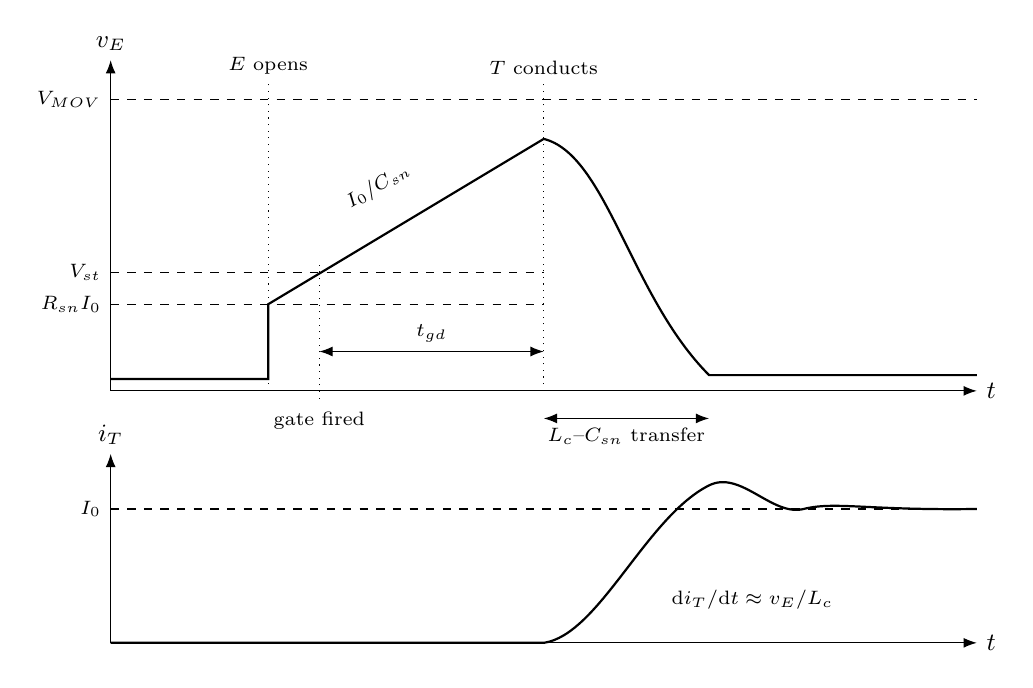
\begin{tikzpicture}[scale=1.0, >=Latex]
  % axes
  \draw[->] (0,0) -- (11,0) node[right, font=\small] {$t$};
  \draw[->] (0,0) -- (0,4.2) node[above, font=\small] {$v_E$};
  % voltage waveform: step, ramp, plateau/turn-on, LC collapse
  \draw[thick] (0,0.15) -- (2,0.15) -- (2,1.1) -- (5.5,3.2) -- (5.5,3.2)
        .. controls (6.3,3.0) and (6.6,1.2) .. (7.6,0.2) -- (11,0.2);
  % levels
  \draw[dashed] (0,1.1) -- (5.5,1.1) node[pos=0, left, font=\scriptsize] {$R_{sn} I_0$};
  \draw[dashed] (0,1.5) -- (5.5,1.5) node[pos=0, left, font=\scriptsize] {$V_{st}$};
  \draw[dashed] (0,3.7) -- (11,3.7) node[pos=0, left, font=\scriptsize] {$V_{MOV}$};
  % times
  \draw[dotted] (2,0) -- (2,3.9) node[above, font=\scriptsize] {$E$ opens};
  \draw[dotted] (2.65,-0.1) -- (2.65,1.6); \node[font=\scriptsize, anchor=north] at (2.65,-0.15) {gate fired};
  \draw[dotted] (5.5,0) -- (5.5,3.9) node[above, font=\scriptsize] {$T$ conducts};
  \draw[<->] (2.65,0.5) -- (5.5,0.5) node[midway, above, font=\scriptsize] {$t_{gd}$};
  \draw[<->] (5.5,-0.35) -- (7.6,-0.35) node[midway, below, font=\scriptsize] {$L_c$--$C_{sn}$ transfer};
  \node[font=\scriptsize, rotate=31] at (3.4,2.6) {$I_0/C_{sn}$};
  % current waveform (offset axis)
  \begin{scope}[yshift=-3.2cm]
    \draw[->] (0,0) -- (11,0) node[right, font=\small] {$t$};
    \draw[->] (0,0) -- (0,2.4) node[above, font=\small] {$i_T$};
    \draw[thick] (0,0) -- (5.5,0) .. controls (6.2,0.1) and (6.8,1.6) .. (7.6,2.0)
          .. controls (8.0,2.2) and (8.4,1.6) .. (8.8,1.7) .. controls (9.2,1.8) and (9.6,1.68) .. (11,1.7);
    \draw[dashed] (0,1.7) -- (11,1.7) node[pos=0, left, font=\scriptsize] {$I_0$};
    \node[font=\scriptsize, anchor=west] at (7.0,0.55) {$\mathrm{d}i_T/\mathrm{d}t \approx v_E/L_c$};
  \end{scope}
\end{tikzpicture}
\caption{Qualitative sequence at the opening of $E$: resistive step of the snubber, linear
rise at $I_0/C_{sn}$, gate fired at $V_{st}$, conduction after $t_{gd}$, transfer of the current
into the thyristor through $L_c$ with the $L_c$--$C_{sn}$ overshoot. The MOV intervenes only if
the thyristor is late.}
\label{fig:timing}
\end{figure}

\subsection{The delay interval: snubber capacitor and MOV}

Between the opening of $E$ and the conduction of the thyristor, i.e.\ the turn-on delay
$t_{gd}$ (\SIrange{1}{3}{\micro s} for a large press-pack with hard gate drive) plus the time to
reach $V_{st}$, the full $I_0$ must flow into something placed across $E$. Two elements share
the task:

\begin{itemize}
\item An RC snubber $C_{sn}$, $R_{sn}$ that turns \eqref{eq:dvdt_par} into a controlled ramp,
      \begin{equation}
        \frac{\mathrm{d}v_E}{\mathrm{d}t} \approx \frac{I_0}{C_{sn}},
        \qquad v_E(t) \approx R_{sn} I_0 + \frac{I_0}{C_{sn}}\,t .
        \label{eq:ramp}
      \end{equation}
      $C_{sn}$ is chosen so that the ramp stays below the critical $\mathrm{d}v/\mathrm{d}t$ of
      the thyristor: the device must be turned on by its gate, not by displacement current, and
      the gate pulse is issued at $V_{st}$ while the voltage continues to rise during $t_{gd}$.
      The resistive step $R_{sn} I_0$ appears instantly; if it exceeds $V_{st}$ the crowbar is
      armed at $t = 0$, which is welcome, but $R_{sn} I_0$ also adds to the voltage reached at
      $t_{gd}$.
\item A MOV in parallel, with knee above the voltage reached at $t_{gd}$ in the nominal
      sequence and clamp level within the blocking capability of the thyristors. In the
      nominal sequence it carries little; it covers a longer delay, a missing gate pulse for a
      few tens of microseconds and the $L_c$ overshoot. It cannot cover a thyristor that never
      fires: with the source connected, the energy at $V_{MOV}$ grows as $V_{MOV} I_0 t$ until
      $S$ opens, tens of kilojoules in tens of milliseconds. Protection against a dead crowbar
      is the fast trip of $S$, Section~\ref{sec:duty}.
\end{itemize}

\subsection{Current transfer: the series reactor}

Once the thyristor conducts, the current transfers from $C_{sn}$ (and the MOV) into the
thyristor branch. Without $L_c$ the loop is the stray inductance of a few hundred nanohenry
and the rate of rise would be
$v_E/L_\sigma \sim \SI{1.4}{kV}/\SI{0.2}{\micro H} = \SI{7}{kA/\micro s}$, far beyond any
phase-control thyristor. A small reactor in the crowbar branch sets
\begin{equation}
  \frac{\mathrm{d}i_T}{\mathrm{d}t} \approx \frac{v_E(t_{gd})}{L_c}, \qquad
  Z_0 = \sqrt{\frac{L_c}{C_{sn}}}, \qquad
  \hat{i}_T \approx I_0 + \frac{v_E(t_{gd})}{Z_0},
  \label{eq:transfer}
\end{equation}
the last term being the $L_c$--$C_{sn}$ exchange overshoot, lightly damped by $R_{sn}$
($\zeta = R_{sn}/2Z_0$). A saturable core is an option: it is a reactor during the transfer and
disappears in continuous conduction. $L_c$ costs nothing in service, since no current flows in
the crowbar branch.

\subsection{Static firing level versus normal transients}
\label{sec:vst}

In service the forward-biased thyristor sees
\begin{equation}
  v_E = R_E\, i_E + L_E\,\frac{\mathrm{d}i_E}{\mathrm{d}t},
  \label{eq:vservice}
\end{equation}
and $V_{arm}$, hence $V_{st}$, must exceed the worst case of \eqref{eq:vservice} with margin.
The resistive term is a few volts. The inductive term depends on where $E$ sits:

\begin{itemize}
\item \emph{Inside the load loop} (in series with $R$, $L$): $i_E$ is the load current, continuous
      through \SI{2}{mH}; at the opening of $S$ it changes at $I_0/\tau \approx \SI{2}{A/\micro s}$
      and the inductive term is negligible.
\item \emph{In the source branch} (in series with $S$, as drawn in Fig.~\ref{fig:system}):
      at the turn-off of $S$ the current through $E$ falls at the IGBT rate, kiloamperes per
      microsecond. With $L_E = \SI{0.5}{\micro H}$ and \SI{3}{kA/\micro s} the inductive term is
      \SI{1.5}{kV}: a passive crowbar with $V_{st}$ of a few hundred volts would fire at every
      opening of $S$. The options are a much higher $V_{st}$ (with $C_{sn}$, MOV and thyristor
      class scaled accordingly), a very low-inductance $E$ and connection, or giving up passive
      firing in favour of a controlled trigger through the external command input.
\end{itemize}

The same applies to any \emph{intended} opening of $E$: a passive crowbar cannot be inhibited.
If $E$ is ever meant to open under current, this scheme does not apply.

\subsection{Duty after firing and clearing}
\label{sec:duty}

After firing, the crowbar is a short in series with the loop; the source keeps driving $I_0$
through it until $S$ opens. Two consequences:

\begin{itemize}
\item The thyristor dissipates $P_T = (V_{T0} + r_T I_0)\,I_0$, about \SI{7.8}{kW} at
      \SI{3600}{A} for the reference device, continuously. With double-side cooling this is
      within its steady-state rating; for a bench that trips $S$ within \SI{100}{ms} the junction
      excursion is a few tens of kelvin and $\int i^2\mathrm{d}t \approx \SI{1.3e6}{A^2 s}$ is
      three orders of magnitude below the device limit. The reference device is oversized on
      voltage (it sees \SI{5}{V} in service and \SI{2}{kV} at most in the event) and adequate
      on current; a lower voltage class with the same wafer would do.
\item The firing must trip $S$: from the model output $M$ in simulation, and in hardware from a
      current transducer in the crowbar branch or from a voltage detector across $E$. Once $S$
      opens, the loop current goes to the dump crowbar of the load, the bypass current decays to
      zero and the thyristor turns off at $I_H$; if $E$ is in the source branch, no current
      flows through it at all after $S$ opens.
\end{itemize}

\subsection{Worked example}
\label{sec:example}

Reference values: $I_0 = \SI{3600}{A}$, $R_E \approx \SI{1.4}{m\ohm}$, thyristors
5STP~26N6500 ($V_{T0} = \SI{1.12}{V}$, $r_T = \SI{0.29}{m\ohm}$, critical
$\mathrm{d}v/\mathrm{d}t$ \SI{1000}{V/\micro s}, $I_{GT} \le \SI{0.4}{A}$), $t_{gd} = \SI{2}{\micro s}$.

\begin{table}[htbp]
\centering
\caption{Worked example of the coordination.}
\label{tab:example}
\small
\begin{tabular}{@{}lp{3.6cm}p{7.6cm}@{}}
\toprule
Quantity & Value & Rule \\
\midrule
$V_{arm}$ & \SI{100}{V} & $\gg R_E I_0 + L_E\,\mathrm{d}i/\mathrm{d}t$ in service (element in load loop) \\
$V_{st}$ & \SI{400}{V} & $V_{arm} + V_{BOD}$; well below MOV knee \\
$C_{sn}$ & \SI{8}{\micro F} & $I_0/C_{sn} = \SI{450}{V/\micro s} <$ critical $\mathrm{d}v/\mathrm{d}t$ \\
$R_{sn}$ & \SI{0.15}{\ohm} & step $R_{sn} I_0 = \SI{540}{V}$ (arms at $t=0$); $\zeta = R_{sn}/2Z_0 \approx 0.1$ \\
$v_E(t_{gd})$ & \SI{1.44}{kV} & $R_{sn} I_0 + (I_0/C_{sn})\,t_{gd}$ \\
MOV & knee $\approx \SI{1.6}{kV}$, clamp $\approx \SI{2}{kV}$ at \SI{3.6}{kA} & idle in the nominal sequence, back-up for a late gate \\
$L_c$ & \SI{5}{\micro H} & $\mathrm{d}i_T/\mathrm{d}t = \SI{1.44}{kV}/\SI{5}{\micro H} = \SI{290}{A/\micro s}$ \\
$Z_0$, $\hat{i}_T$ & \SI{0.79}{\ohm}, $\approx \SI{5.4}{kA}$ & overshoot $v_E/Z_0 \approx \SI{1.8}{kA}$ on top of $I_0$ \\
$E_{C_{sn}}$ & \SI{8}{J} & $\tfrac12 C_{sn} v_E^2$, dissipated in $R_{sn}$ and thyristor \\
$P_T$ & \SI{7.8}{kW} & $(V_{T0} + r_T I_0) I_0$ until $S$ opens \\
$\int i^2 \mathrm{d}t$ (\SI{100}{ms}) & \SI{1.3e6}{A^2 s} & vs.\ $\sim\SI{2e7}{A^2 s}$ of the device \\
Thyristor class & \SIrange{2.8}{4.5}{kV} sufficient & $V_{RRM} \ge$ MOV clamp with margin; \SI{6.5}{kV} reference oversized \\
\bottomrule
\end{tabular}
\normalsize
\end{table}

With these values the voltage crosses $V_{st}$ at $t = 0$ because of the resistive step,
the thyristor conducts at \SI{2}{\micro s} with \SI{1.44}{kV} across it, and the current is
in the thyristor \SI{15}{\micro s} later. The MOV is a back-up. If $C_{sn}$ is removed and
only the MOV is kept, $v_E$ reaches the clamp within nanoseconds at a rate that exceeds the
critical $\mathrm{d}v/\mathrm{d}t$ by orders of magnitude: the thyristor still turns on, but by
displacement current over a random area, and the model flags it with $|M| = 4$.

% ==========================================================================
\section{Functional Simscape component \texttt{crowbar\_bidir}}
% ==========================================================================

\subsection{Interface}

Two electrical conserving ports \texttt{p} (left) and \texttt{n} (right); $T_1$ conducts
p$\to$n, $T_2$ conducts n$\to$p. Physical-signal input \texttt{G} (bottom): external fire
command, dimensionless, fires the forward-biased thyristor when above 0.5; connect a PS
Constant 0 if unused. Physical-signal output \texttt{M} (top): signed state code, zero while
blocking, sign equal to the conduction direction ($+1$ for $T_1$), magnitude equal to the
trigger source of Table~\ref{tab:M}.

\begin{table}[htbp]
\centering
\caption{Trigger source codes reported on $|M|$ (priority order).}
\label{tab:M}
\begin{tabular}{@{}clp{8.5cm}@{}}
\toprule
$|M|$ & Source & Meaning \\
\midrule
1 & static (BOD) & gate current reached $I_{GT}$ with the BOD conducting: nominal firing at $V_{st}$ \\
2 & dynamic ($C_g$) & gate current reached $I_{GT}$ through $C_g$ alone, above $V_{arm}$ \\
3 & external & command \texttt{G} $> 0.5$ \\
4 & intrinsic $\mathrm{d}v/\mathrm{d}t$ & $\mathrm{d}v/\mathrm{d}t$ exceeded the critical value with $v > V_{min}$ before any gate path: uncontrolled turn-on, increase $C_{sn}$ or lower $V_{st}$ \\
5 & breakover & $v$ exceeded $V_{BO}$ before any gate path: uncontrolled turn-on \\
\bottomrule
\end{tabular}
\end{table}

\subsection{Equations}

Main branch, with $i$ positive p$\to$n and $d \in \{+1,-1\}$ the conduction direction:
\begin{align}
  \text{blocking:}& \quad i = G_{off}\, v, \\
  \text{conducting:}& \quad v = d\, V_{T0} + r_T\, i .
\end{align}
Trigger networks ($k = 1$ for $T_1$ with $v_1 = v$, $k = 2$ for $T_2$ with $v_2 = -v$):
\begin{align}
  i_{d,k} &= \begin{cases}
    (v_k - V_{arm} - v_{C,k})/R_{ser} & v_k - V_{arm} - v_{C,k} > 0 \\
    (v_k - V_{arm} - v_{C,k})\, G_{D1,off} & \text{otherwise}
  \end{cases} \\
  C_g\,\frac{\mathrm{d}v_{C,k}}{\mathrm{d}t} &= i_{d,k} - \frac{v_{C,k}}{R_C} - i_{st,k},
  \qquad i_{st,k} = \frac{\max(v_{C,k} - V_{BOD},\,0)}{R_s}, \quad V_{BOD} = V_{st} - V_{arm}, \\
  v_{gk,k} &= V_{GT}\tanh\!\left(\frac{i_{d,k} R_{GK}}{V_{GT}}\right), \qquad
  i_{j,k} = i_{d,k} - \frac{v_{gk,k}}{R_{GK}} .
\end{align}
The junction current $i_{j,k}$ reaches $I_{GT}$ when $i_{d,k} = I_{GT} + V_{GT}/R_{GK}$.
The terminal current is $i_t = i + i_{d,1} - i_{d,2}$. The rate of change of $v$ is estimated
with a first-order filter of time constant $\tau_f$, so that no derivative appears in event
conditions. Two integrators, $\int i^2 \mathrm{d}t$ and $\int v\,i\,\mathrm{d}t$, are exposed
for the thermal check of Section~\ref{sec:duty}.

\subsection{State machine}

Five event variables: \texttt{on}, \texttt{dir} ($d$), \texttt{armed}, \texttt{latched},
\texttt{mode}, plus the trigger time \texttt{t\_trig}.

\begin{enumerate}
\item \textbf{Arming.} While blocking and not armed, the first of the conditions of
      Table~\ref{tab:M} that becomes true for $T_1$ ($v > 0$) or $T_2$ ($v < 0$) sets
      \texttt{armed} $= 1$, \texttt{dir}, \texttt{mode} and records the time.
\item \textbf{Turn-on.} At \texttt{t\_trig} $+ t_{gd}$: if $d\,v > 0$ still holds, \texttt{on} $=1$;
      otherwise the arming is cancelled (polarity reversed during the delay).
\item \textbf{Latching.} \texttt{latched} $= 1$ when $d\,i > I_L$.
\item \textbf{Turn-off.} \texttt{on} $= 0$ when $d\,i < I_H$ after latching. The latch flag
      prevents a spurious turn-off at the switching instant, when the current starts from zero.
\end{enumerate}

All trigger sources, including the intrinsic ones, go through the same delay: the code on $M$
records which condition came first, which is the design information needed.

\subsection{Parameters}

\begin{table}[htbp]
\centering
\caption{Parameters and defaults of \texttt{crowbar\_bidir}.}
\label{tab:par}
\begin{tabular}{@{}llll@{}}
\toprule
Group & Name & Default & Meaning \\
\midrule
On-state & \texttt{Vt0}, \texttt{rT} & \SI{1.12}{V}, \SI{0.29}{m\ohm} & PWL on-state \\
 & \texttt{Goff} & \SI{1e-6}{S} & off-state conductance, both polarities \\
 & \texttt{Il}, \texttt{Ih} & \SI{2}{A}, \SI{1}{A} & latching, holding current \\
 & \texttt{tgd} & \SI{2}{\micro s} & turn-on delay ($>0$) \\
Gate & \texttt{Igt}, \texttt{Vgt}, \texttt{Rgk} & \SI{0.4}{A}, \SI{3}{V}, \SI{10}{\ohm} & trigger current/voltage, $R_{GK}$ \\
Network & \texttt{Varm}, \texttt{Vst} & \SI{100}{V}, \SI{400}{V} & arming and static firing levels \\
 & \texttt{Cg}, \texttt{Rc} & \SI{1}{nF}, \SI{22}{k\ohm} & dynamic path, reset \\
 & \texttt{Rs}, \texttt{Rser} & \SI{100}{\ohm}, \SI{11}{\ohm} & static path resistor, loop series resistance \\
 & \texttt{Gd1off} & \SI{1e-9}{S} & $D_1$ off-state conductance \\
Intrinsic & \texttt{dvdt\_crit}, \texttt{Vmin} & \SI{1e9}{V/s}, \SI{50}{V} & intrinsic $\mathrm{d}v/\mathrm{d}t$ firing \\
 & \texttt{Vbo}, \texttt{tau\_f} & \SI{7800}{V}, \SI{50}{ns} & breakover, $\mathrm{d}v/\mathrm{d}t$ sensing \\
\bottomrule
\end{tabular}
\end{table}

Not modelled: plasma spreading and $\mathrm{d}i/\mathrm{d}t$ limits, reverse recovery, $t_q$,
thermal feedback on $V_{T0}$ and $r_T$. The reactor, the snubber and the MOV are external
blocks, so that their values can be swept.

% ==========================================================================
\section{Simulation test procedure}
% ==========================================================================

Model $E$ as a resistor $R_E$ in series with an ideal switch that opens at $t_0$ with the
full $I_0$ established, a stray capacitance $C_{par}$ of a few nanofarad across it, the RC
snubber, the MOV (the existing varistor or \texttt{tvs\_clamp} model), and the crowbar
branch $L_c$ + \texttt{crowbar\_bidir}. Fixed step \SI{10}{ns} is adequate
($C_g R_{ser} \approx \SI{10}{ns}$, $\tau_f = \SI{50}{ns}$).

\begin{enumerate}
\item \textbf{Nominal event.} Record $v_E$, $i_T$, $M$, the MOV current and $i_{j,1}$.
      Expected: arming at $t_0$ (resistive step), $M = +1$ at $t_0 + t_{gd}$, peak $v_E$ per
      Table~\ref{tab:example}, $\mathrm{d}i_T/\mathrm{d}t$ and overshoot per \eqref{eq:transfer},
      MOV current negligible.
\item \textbf{Snubber removed.} Keep the MOV only: $M$ should read $+4$, the sign that the
      design relies on displacement-current turn-on. Reinstate $C_{sn}$ and find the minimum
      value that restores $M = +1$; compare with $I_0/(\mathrm{d}v/\mathrm{d}t)_{crit}$.
\item \textbf{Delay sweep.} $t_{gd}$ from \SIrange{1}{5}{\micro s}: $v_E(t_{gd})$ must stay below
      the MOV knee; note where the MOV starts to share current.
\item \textbf{Reactor sweep.} $L_c$ from \SIrange{1}{10}{\micro H}: read $\mathrm{d}i_T/\mathrm{d}t$
      in the first microseconds and the overshoot against the device rating.
\item \textbf{Reverse polarity.} Repeat with the current reversed (or $E$ in the other
      orientation): $M = -1$, symmetric waveforms.
\item \textbf{False-firing margin.} With $E$ closed, apply the normal bench sequence
      (closing and opening of $S$, firing of the dump crowbar) and check that
      $\max |v_E| < V_{arm}$ with margin and that $M$ stays 0; if $E$ is in the source branch,
      include the element inductance $L_E$ explicitly.
\item \textbf{Clearing.} After firing, open $S$ per the bench logic and verify that $i_T$
      decays to zero, \texttt{on} drops at $I_H$ and \texttt{i2t}, \texttt{Ed} match the
      thermal estimate.
\end{enumerate}

% ==========================================================================
\section{Conclusions}
% ==========================================================================

A bidirectional, passively fired thyristor crowbar is a sound way to protect a structurally
short element against an unwanted opening at \SI{3600}{A}: it needs no auxiliary power, fires
within microseconds in either polarity and carries the full current until the main switch
clears. Its design differs from the dump crowbar in three points that the coordination of
Section~\ref{sec:coord} addresses: an arming threshold well above the service transients of the
element (whose position in the loop decides how large they are), a snubber capacitor and MOV
that hold the voltage during the turn-on delay while keeping the $\mathrm{d}v/\mathrm{d}t$ below
the critical value, and a small series reactor that keeps the current transfer within the
$\mathrm{d}i/\mathrm{d}t$ capability of the device. The crowbar is a latch: its firing must trip
the main switch, and it cannot be inhibited, so it is only applicable to an element that is
never meant to open under current. The functional component \texttt{crowbar\_bidir} reproduces
the trigger paths, the delay and the latch, and reports on $M$ which mechanism fired first,
which is the quantity to watch when sizing $C_{sn}$ and $V_{st}$.

% ==========================================================================
\begin{thebibliography}{9}

\bibitem{selftrig}
D.~Bagnara, ``Crowbar thyristor for the 3~kV / 3600~A static-switch test bench: device selection
and passive self-triggering gate circuit,'' technical note \texttt{crowbar\_thyristor\_selftrigger},
Rev.~00, 2026.

\bibitem{ds26n6500}
Hitachi Energy (formerly ABB Semiconductors), ``Phase Control Thyristor 5STP~26N6500,'' data sheet.

\bibitem{baliga}
B.~J. Baliga, \emph{Fundamentals of Power Semiconductor Devices}. New York: Springer, 2008,
ch.~8 (Thyristors).

\bibitem{bodpatent}
``Protective circuitry for a thyristor,'' U.S. Patent 4\,651\,251 (break-over diode protective firing).

\bibitem{arrillaga}
J.~Arrillaga, \emph{High Voltage Direct Current Transmission}, 2nd ed. London: IEE, 1998
(thyristor valves, protective firing).

\bibitem{mov}
D.~Bagnara, ``EPCOS SIOV-B80K680 block varistor: operating characteristics and application
sizing,'' technical note, 2026.

\end{thebibliography}

\end{document}
